\documentclass[a4paper]{article}

%% Language and font encodings
\usepackage[english]{babel}
\usepackage[utf8x]{inputenc}
\usepackage[T1]{fontenc}
\usepackage{amsmath}

%% Sets page size and margins
\usepackage[a4paper,top=3cm,bottom=2cm,left=3cm,right=3cm,marginparwidth=1.75cm]{geometry}

%% Useful packages
\usepackage{amsmath}
\usepackage{graphicx}
\usepackage[colorinlistoftodos]{todonotes}
\usepackage[colorlinks=true, allcolors=blue]{hyperref}

\title{CS 440 Fall 2018 Homework Assignment 1}
\author{Rafal Stapinski}

\begin{document}
\maketitle


\section{}
(P(-5) $\lor$ P(-3) $\lor$ P(-1) $\lor$ P(-1) $\lor$ P(3))

\section{}

($\neg$∃x∀y(P(x,y) → Q(x,y))) → (∀x∀y∃z(P(x,y) → $\neg$P(y,z)))

\section{}

The divisors or 123 are 1, 3, 41, 123 found by keeping whole quotients of divisions of 123 from 1 to $\sqrt[]{123}$.
The divisors of 46 are 1, 2, 23, 46 found by keeping whole quotients of divisions of 46 from 1 to $\sqrt[]{46}$.
The greated common divisor is therefore 1.
gcd(46, 123) = 1


\section{}

A complete graph with n vertices has the highest amount of edges for any graph with n vertices
Base case: n = 1, there are |E| = 0 edges, n=2, there are |E| = 1 edges.
For each additional vertex, there will be n new edges as the new vertex will make n connections to each of the n existing vertices. Suppose a complete graph with n vertices has |E| edges. If a vertex is added, there will be n+1 vertices and |E| + n edges. 


\section{}

$P_4^9$

\section{}

Complete bipartite graphs: $K_{1,n}$ and $K_{2,n}$
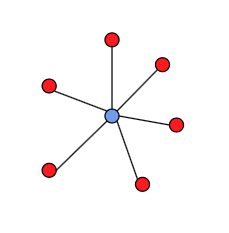
\includegraphics[scale=.5]{k1n.png}
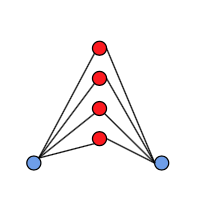
\includegraphics[scale=.5]{k2n.png}

\noindent Complete graphs: $K_1$, $K_2$, $K_3$, and $K_4$

\includegraphics[scale=.6]{k1.png}
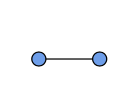
\includegraphics[scale=.6]{k2.png}
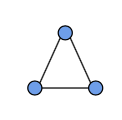
\includegraphics[scale=.6]{k3.png}
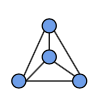
\includegraphics[scale=.6]{k4.png}

\section{}
The smallest complete graph that is non-planar is the pentatope graph $K_5$. Looking at the graph $K_4$ which can only be drawn as a planar graph as a triangular set of vertices with the fourth being in the middle of them as shown above. In this case, there are two places in which a new vertex can be placed to make this a $K_5$ graph. The first is in any of the three internal triangles. In this case, it is obvious that connections to two of the four existing vertices would require edges to cross. The second location for a new vertex is outside the graph entirely. Here, it is also clear that two of the four existing vertices would require edges that cross existing edges. 

\section{}
\subsection{}
at most n
\subsection{}
there are $\prod_{k=1}^{n}{\frac{1}{1 - n^k}}$
\subsection{}
n * m - (n + m)

\end{document}